% Supervisor Usage Guide
% A complete introduction to OTP supervisor with architecture diagrams and examples.
% Compile with: xelatex supervisor_architecture.tex (run twice for TOC)
\documentclass[a4paper,11pt]{article}

% ============================================================
% Packages
% ============================================================
\usepackage{fontspec}
\usepackage{xeCJK}
\setCJKmainfont[BoldFont=STHeiti, ItalicFont=STKaiti]{STSong}
\setCJKsansfont{STHeiti}
\setCJKmonofont{STFangsong}

\usepackage[margin=2.5cm]{geometry}
\usepackage{graphicx}
\usepackage{xcolor}
\usepackage{hyperref}
\usepackage{listings}
\usepackage{booktabs}
\usepackage{longtable}
\usepackage{enumitem}
\usepackage{tikz}
\usepackage{tcolorbox}
\usepackage{fancyhdr}
\usepackage{titlesec}
\usepackage{amsmath}
\usepackage{amssymb}
\usepackage{float}
\usepackage{pifont}

\usetikzlibrary{arrows.meta, positioning, shapes.geometric, fit, calc, backgrounds, decorations.pathreplacing}

\tcbuselibrary{listings, skins, breakable}

% ============================================================
% Color Definitions
% ============================================================
\definecolor{erlred}{HTML}{A4070A}
\definecolor{erlblue}{HTML}{2B5EA7}
\definecolor{erlgreen}{HTML}{2E7D32}
\definecolor{erlyellow}{HTML}{F9A825}
\definecolor{erlpurple}{HTML}{6A1B9A}
\definecolor{erlmodule}{HTML}{D84315}
\definecolor{erlinit}{HTML}{00897B}
\definecolor{erlpid}{HTML}{E65100}
\definecolor{erlname}{HTML}{6A1B9A}
\definecolor{codebg}{HTML}{F5F5F5}
\definecolor{codeborder}{HTML}{CCCCCC}
\definecolor{tipbg}{HTML}{E8F5E9}
\definecolor{warnbg}{HTML}{FFF3E0}
\definecolor{notebg}{HTML}{E3F2FD}
\definecolor{darkgray}{HTML}{333333}

% ============================================================
% Hyperref Setup
% ============================================================
\hypersetup{
    colorlinks=true,
    linkcolor=erlblue,
    urlcolor=erlpurple,
    citecolor=erlgreen,
    pdftitle={Supervisor 用法指南},
    pdfauthor={Erlang OTP Tutorial},
    bookmarksnumbered=true,
}

% ============================================================
% Code Listing Style
% ============================================================
\lstdefinelanguage{erlang}{
    morekeywords={module, export, import, behaviour, behavior, spec, type,
        record, define, include, ifdef, ifndef, else, endif, undef,
        case, of, end, if, receive, after, when, fun, try, catch, throw,
        begin, spawn, spawn_link, register, self, send, ok, error,
        true, false, undefined, infinity, timeout, noreply, reply, stop,
        hibernate, ignore, normal, process_flag, trap_exit, monitor_node,
        permanent, transient, temporary, worker, supervisor,
        one_for_one, one_for_all, rest_for_one, simple_one_for_one},
    sensitive=true,
    morecomment=[l]{\%},
    morestring=[b]",
    morestring=[b]',
}

\lstdefinestyle{erlangstyle}{
    language=erlang,
    basicstyle=\ttfamily\small,
    keywordstyle=\color{erlblue}\bfseries,
    commentstyle=\color{erlgreen}\itshape,
    stringstyle=\color{erlred},
    numberstyle=\tiny\color{gray},
    numbers=left,
    numbersep=8pt,
    backgroundcolor=\color{codebg},
    frame=single,
    rulecolor=\color{codeborder},
    breaklines=true,
    breakatwhitespace=true,
    tabsize=4,
    showstringspaces=false,
    captionpos=b,
    xleftmargin=1.5em,
    framexleftmargin=1em,
    aboveskip=1em,
    belowskip=0.8em,
}

\lstdefinestyle{shellstyle}{
    basicstyle=\ttfamily\small\color{white},
    backgroundcolor=\color{darkgray},
    rulecolor=\color{darkgray},
    frame=single,
    breaklines=true,
    showstringspaces=false,
    xleftmargin=1.5em,
    framexleftmargin=1em,
    aboveskip=1em,
    belowskip=0.8em,
}

\lstset{style=erlangstyle}

% ============================================================
% Custom tcolorbox Environments
% ============================================================
\newtcolorbox{tipbox}[1][]{
    colback=tipbg, colframe=erlgreen!80!black,
    fonttitle=\bfseries, title={#1},
    arc=2mm, boxrule=0.8pt,
    left=6pt, right=6pt, top=4pt, bottom=4pt,
    breakable,
}

\newtcolorbox{warnbox}[1][]{
    colback=warnbg, colframe=erlyellow!80!black,
    fonttitle=\bfseries, title={#1},
    arc=2mm, boxrule=0.8pt,
    left=6pt, right=6pt, top=4pt, bottom=4pt,
    breakable,
}

\newtcolorbox{notebox}[1][]{
    colback=notebg, colframe=erlblue!80!black,
    fonttitle=\bfseries, title={#1},
    arc=2mm, boxrule=0.8pt,
    left=6pt, right=6pt, top=4pt, bottom=4pt,
    breakable,
}

% ============================================================
% Header / Footer
% ============================================================
\pagestyle{fancy}
\fancyhf{}
\fancyhead[L]{\small\textit{Supervisor 用法指南}}
\fancyhead[R]{\small\textit{Erlang/OTP}}
\fancyfoot[C]{\thepage}
\renewcommand{\headrulewidth}{0.4pt}

% ============================================================
% Title Formatting
% ============================================================
\titleformat{\section}
    {\LARGE\bfseries\color{erlblue}}
    {\thesection}{1em}{}[\vspace{-0.5em}\rule{\textwidth}{0.8pt}]

\titleformat{\subsection}
    {\Large\bfseries\color{erlblue!80!black}}
    {\thesubsection}{0.8em}{}

\titleformat{\subsubsection}
    {\large\bfseries\color{erlblue!60!black}}
    {\thesubsubsection}{0.6em}{}

% ============================================================
% Document Begin
% ============================================================
\begin{document}

% ---- Title Page ----
\begin{titlepage}
\centering
\vspace*{3cm}

{\fontsize{42}{48}\selectfont\bfseries\color{erlblue} supervisor}\\[12pt]
{\fontsize{24}{28}\selectfont\color{erlblue!70!black} 用法指南}

\vspace{2cm}

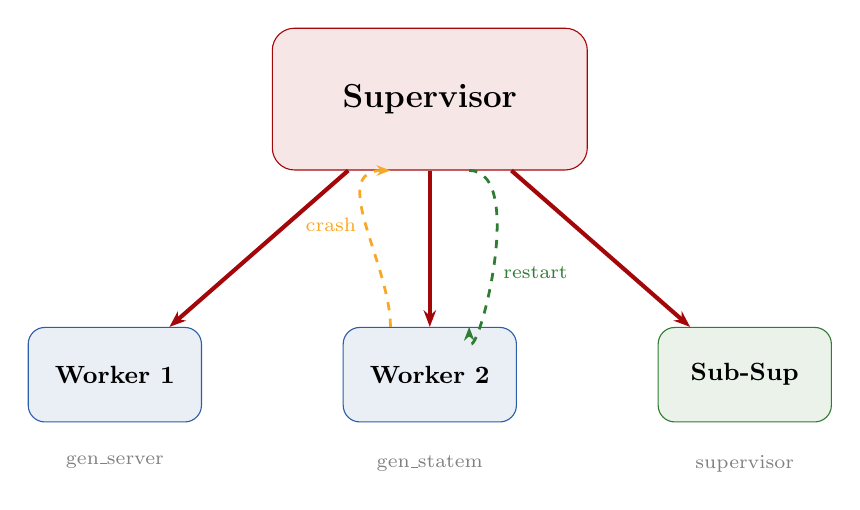
\begin{tikzpicture}
    % Supervisor
    \node[draw=erlred, fill=erlred!10, rounded corners=8pt, minimum width=4cm, minimum height=1.8cm, font=\large\bfseries] (sup) at (4,0) {Supervisor};

    % Workers
    \node[draw=erlblue, fill=erlblue!10, rounded corners=6pt, minimum width=2.2cm, minimum height=1.2cm, font=\small\bfseries] (w1) at (0,-3.5) {Worker 1};
    \node[draw=erlblue, fill=erlblue!10, rounded corners=6pt, minimum width=2.2cm, minimum height=1.2cm, font=\small\bfseries] (w2) at (4,-3.5) {Worker 2};
    \node[draw=erlgreen, fill=erlgreen!10, rounded corners=6pt, minimum width=2.2cm, minimum height=1.2cm, font=\small\bfseries] (w3) at (8,-3.5) {Sub-Sup};

    % Links
    \draw[-{Stealth[length=6pt]}, line width=1.5pt, erlred] (sup) -- (w1);
    \draw[-{Stealth[length=6pt]}, line width=1.5pt, erlred] (sup) -- (w2);
    \draw[-{Stealth[length=6pt]}, line width=1.5pt, erlred] (sup) -- (w3);

    % Crash & restart
    \draw[-{Stealth[length=5pt]}, line width=1pt, erlyellow, dashed] ([xshift=-5mm]w2.north) .. controls ++(0,0.8) and ++(-0.8,0) .. node[left, font=\scriptsize\color{erlyellow}] {crash} ([xshift=-5mm]sup.south);
    \draw[-{Stealth[length=5pt]}, line width=1pt, erlgreen, dashed] ([xshift=5mm]sup.south) .. controls ++(0.8,0) and ++(0,-0.8) .. node[right, font=\scriptsize\color{erlgreen}] {restart} ([xshift=5mm]w2.north);

    \node[below=3mm of w1, font=\scriptsize\color{gray}] {gen\_server};
    \node[below=3mm of w2, font=\scriptsize\color{gray}] {gen\_statem};
    \node[below=3mm of w3, font=\scriptsize\color{gray}] {supervisor};
\end{tikzpicture}

\vspace{3cm}

{\large\color{darkgray} 以 frequency\_sup 为例，从原理到实践}

\vspace{1cm}

{\normalsize\color{gray} Erlang/OTP $\cdot$ Supervision Tree $\cdot$ Fault Tolerance}

\vfill
{\small\today}
\end{titlepage}

% ---- Table of Contents ----
\newpage
\tableofcontents
\newpage


% ============================================================
% Section 1: Overview
% ============================================================
\section{概述}

\subsection{什么是 Supervisor？}

\texttt{supervisor} 是 OTP 框架中的\textbf{监督者}行为模式（behavior），负责启动、监控和重启子进程。它是 Erlang ``Let it crash'' 哲学的核心实现，通过监督树（supervision tree）构建容错系统。

\begin{tipbox}[核心思想]
\textbf{Supervisor = Process Monitor + Restart Strategy + Child Specification}

\begin{itemize}[leftmargin=1.5em]
    \item \textbf{Process Monitor}：监控子进程的生死状态
    \item \textbf{Restart Strategy}：定义子进程崩溃时的重启策略（one\_for\_one、one\_for\_all、rest\_for\_one、simple\_one\_for\_one）
    \item \textbf{Child Specification}：描述每个子进程的启动方式、重启类型、关闭策略等
    \item 开发者只需实现 \texttt{init/1} 回调函数
\end{itemize}
\end{tipbox}

\subsection{为什么需要 Supervisor？}

在没有 supervisor 之前，我们需要手动实现进程监控和重启逻辑：

\begin{lstlisting}[style=erlangstyle, caption={手动实现的 my\_supervisor.erl}]
-module(my_supervisor).
-export([start/2, init/1, stop/1]).

start(Name, ChildSpecList) ->
    register(Name, Pid = spawn(?MODULE, init, [ChildSpecList])),
    {ok, Pid}.

init(ChildSpecList) ->
    process_flag(trap_exit, true),
    loop(start_children(ChildSpecList)).

start_children(ChildSpecList) ->
    [{element(2, apply(M,F,A)), {M,F,A}}
     || {M,F,A} <- ChildSpecList].

loop(ChildList) ->
    receive
        {'EXIT', Pid, normal} ->
            loop(lists:keydelete(Pid, 1, ChildList));
        {'EXIT', Pid, _Reason} ->
            NewChildList = restart_child(Pid, ChildList),
            loop(NewChildList);
        stop ->
            terminate(ChildList)
    end.

restart_child(Pid, ChildList) ->
    {Pid, {M,F,A}} = lists:keyfind(Pid, 1, ChildList),
    {ok, NewPid} = apply(M,F,A),
    lists:keyreplace(Pid, 1, ChildList, {NewPid, {M,F,A}}).

terminate(ChildList) ->
    lists:foreach(
        fun({Pid, _}) -> exit(Pid, kill) end,
        ChildList).
\end{lstlisting}

\begin{notebox}[手动实现的问题]
\begin{itemize}[leftmargin=1.5em]
    \item 只有最简单的重启策略（逐个重启）
    \item 没有重启频率限制（可能无限重启）
    \item 没有优雅关闭（直接 kill）
    \item 没有动态子进程管理
    \item 没有与 OTP 工具链集成（sys、observer 等）
\end{itemize}
\end{notebox}

OTP 的 \texttt{supervisor} 行为模式解决了所有这些问题，提供了生产级别的进程监控能力。

\subsection{通用代码 vs 专用代码}

\begin{table}[H]
\centering
\begin{tabular}{@{}ll@{}}
\toprule
\textbf{通用代码（supervisor 模块）} & \textbf{专用代码（你的回调模块）} \\
\midrule
启动/停止 supervisor 进程 & 子进程规格（child spec） \\
监控子进程（trap\_exit） & 重启策略选择 \\
按策略重启子进程 & 子进程的启动函数 \\
重启频率限制 & 子进程的初始化参数 \\
优雅关闭子进程 & 关闭超时设置 \\
动态添加/删除子进程 & --- \\
与 sys/observer 集成 & --- \\
\bottomrule
\end{tabular}
\caption{通用代码 vs 专用代码}
\end{table}

\subsection{OTP 源码中的工作流}

\begin{tcolorbox}[colback=codebg, colframe=codeborder, arc=2mm, boxrule=0.5pt,
                  title={\textbf{supervisor.erl --- Work Flow}},
                  fonttitle=\bfseries\ttfamily, width=\textwidth]
\small\ttfamily
\begin{tabular}{@{}lcl@{}}
supervisor module &  & Callback module \\
\textsf{-{}-{}-{}-{}-{}-{}-{}-{}-{}-{}-{}-{}-{}-{}-{}-{}-} & & \textsf{-{}-{}-{}-{}-{}-{}-{}-{}-{}-{}-{}-{}-{}-{}-} \\
supervisor:start\_link & -{}-{}-{}-{}-> & Module:init/1 \\
 & & \quad returns \{ok, \{SupFlags, ChildSpecs\}\} \\
supervisor:start\_child & & (dynamic child) \\
supervisor:terminate\_child & & (stop child) \\
supervisor:restart\_child & & (restart stopped child) \\
supervisor:delete\_child & & (remove child spec) \\
supervisor:which\_children & & (list children) \\
supervisor:count\_children & & (count children) \\
\end{tabular}
\end{tcolorbox}


% ============================================================
% Section 2: Supervision Tree Architecture
% ============================================================
\section{监督树架构}

\subsection{监督树的层次结构}

Erlang/OTP 应用程序通常组织为树形结构，supervisor 作为内部节点，worker 进程作为叶子节点：

\begin{figure}[H]
\centering
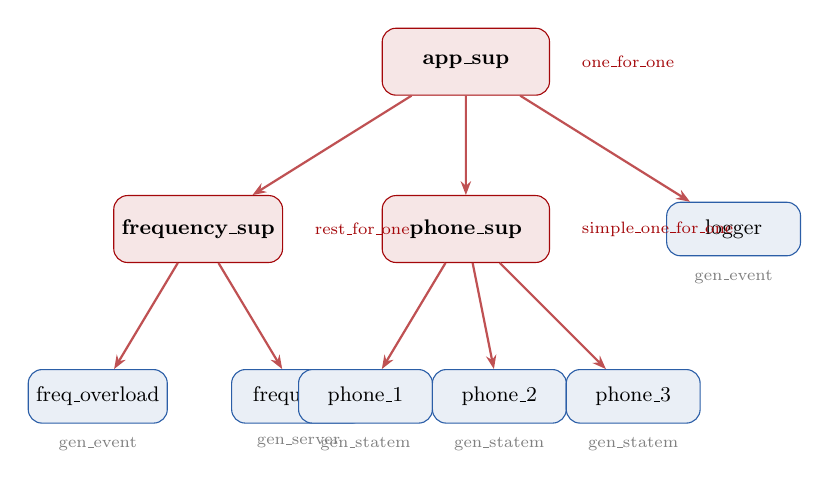
\begin{tikzpicture}[scale=0.85, every node/.style={scale=0.85},
    sup/.style={draw=erlred, fill=erlred!10, rounded corners=5pt,
                minimum width=2.5cm, minimum height=1cm, font=\small\bfseries},
    wrk/.style={draw=erlblue, fill=erlblue!10, rounded corners=5pt,
                minimum width=2cm, minimum height=0.8cm, font=\small},
    link/.style={-{Stealth[length=5pt]}, thick, erlred!70},
]
    % Top-level supervisor
    \node[sup] (top) at (5, 0) {app\_sup};

    % Second level
    \node[sup] (freq_sup) at (1, -2.5) {frequency\_sup};
    \node[sup] (phone_sup) at (5, -2.5) {phone\_sup};
    \node[wrk] (logger) at (9, -2.5) {logger};

    % Third level - frequency_sup children
    \node[wrk] (overload) at (-0.5, -5) {freq\_overload};
    \node[wrk] (freq) at (2.5, -5) {frequency};

    % Third level - phone_sup children
    \node[wrk] (p1) at (3.5, -5) {phone\_1};
    \node[wrk] (p2) at (5.5, -5) {phone\_2};
    \node[wrk] (p3) at (7.5, -5) {phone\_3};

    % Links
    \draw[link] (top) -- (freq_sup);
    \draw[link] (top) -- (phone_sup);
    \draw[link] (top) -- (logger);
    \draw[link] (freq_sup) -- (overload);
    \draw[link] (freq_sup) -- (freq);
    \draw[link] (phone_sup) -- (p1);
    \draw[link] (phone_sup) -- (p2);
    \draw[link] (phone_sup) -- (p3);

    % Labels
    \node[font=\scriptsize\color{gray}, below=2pt of overload] {gen\_event};
    \node[font=\scriptsize\color{gray}, below=2pt of freq] {gen\_server};
    \node[font=\scriptsize\color{gray}, below=2pt of p1] {gen\_statem};
    \node[font=\scriptsize\color{gray}, below=2pt of p2] {gen\_statem};
    \node[font=\scriptsize\color{gray}, below=2pt of p3] {gen\_statem};
    \node[font=\scriptsize\color{gray}, below=2pt of logger] {gen\_event};

    % Annotations
    \node[font=\scriptsize\color{erlred}, right=3mm of top] {one\_for\_one};
    \node[font=\scriptsize\color{erlred}, right=3mm of freq_sup] {rest\_for\_one};
    \node[font=\scriptsize\color{erlred}, right=3mm of phone_sup] {simple\_one\_for\_one};
\end{tikzpicture}
\caption{典型的 OTP 监督树结构}
\label{fig:supervision-tree}
\end{figure}

\subsection{启动流程}

supervisor 的启动是\textbf{同步的、自顶向下的}：

\begin{enumerate}[leftmargin=2em]
    \item 调用 \texttt{supervisor:start\_link(Name, Module, Args)}
    \item supervisor 进程创建，调用 \texttt{Module:init(Args)}
    \item \texttt{init/1} 返回 \texttt{\{ok, \{SupFlags, ChildSpecs\}\}}
    \item supervisor 按照 ChildSpecs 列表\textbf{从左到右依次}启动子进程
    \item 每个子进程启动成功后才启动下一个
    \item 所有子进程启动完成后，\texttt{start\_link} 返回 \texttt{\{ok, Pid\}}
\end{enumerate}

\begin{warnbox}[注意：启动顺序很重要]
子进程按照 ChildSpecs 列表中的\textbf{顺序}启动。如果子进程之间有依赖关系（如 \texttt{frequency} 依赖 \texttt{freq\_overload}），必须确保被依赖的进程排在前面。
\end{warnbox}

\subsection{关闭流程}

supervisor 的关闭是\textbf{与启动顺序相反的}：

\begin{enumerate}[leftmargin=2em]
    \item supervisor 收到关闭信号
    \item 按照 ChildSpecs 列表的\textbf{逆序}逐个关闭子进程
    \item 对每个子进程：发送 \texttt{exit(Child, shutdown)} 信号
    \item 等待子进程在 \texttt{Shutdown} 超时内终止
    \item 如果超时未终止，强制 \texttt{exit(Child, kill)}
    \item 所有子进程关闭后，supervisor 自身终止
\end{enumerate}


% ============================================================
% Section 3: init/1 Return Value
% ============================================================
\section{init/1 回调函数}

\texttt{init/1} 是 supervisor 唯一需要实现的回调函数，返回监督规格：

\begin{lstlisting}[style=erlangstyle]
init(Args) ->
    {ok, {SupFlags, ChildSpecs}}
  | ignore.
\end{lstlisting}

\subsection{SupFlags --- 监督标志}

\subsubsection{元组格式（向后兼容）}

\begin{lstlisting}[style=erlangstyle]
SupFlags = {Strategy, Intensity, Period}
%% Strategy  = one_for_one | one_for_all
%%           | rest_for_one | simple_one_for_one
%% Intensity = integer() >= 0   (max restarts)
%% Period    = integer() >= 1   (time window in seconds)
\end{lstlisting}

\subsubsection{Map 格式（OTP 18+，推荐）}

\begin{lstlisting}[style=erlangstyle]
SupFlags = #{
    strategy => one_for_one,      %% Restart strategy
    intensity => 2,               %% Max 2 restarts
    period => 3600,               %% Within 3600 seconds
    auto_shutdown => never        %% OTP 24+
}.
\end{lstlisting}

\begin{notebox}[重启频率限制]
如果在 \texttt{Period} 秒内重启次数超过 \texttt{Intensity}，supervisor 自身会终止（并向上级 supervisor 报告）。这防止了无限重启循环。

例如 \texttt{intensity => 2, period => 3600} 表示：在 3600 秒内最多允许 2 次重启，第 3 次重启时 supervisor 自身终止。
\end{notebox}

\subsection{ChildSpec --- 子进程规格}

\subsubsection{元组格式（向后兼容）}

\begin{lstlisting}[style=erlangstyle]
ChildSpec = {Id, StartFunc, Restart, Shutdown, Type, Modules}
%% Id        = term()              Unique identifier
%% StartFunc = {M, F, A}           Start function
%% Restart   = permanent | transient | temporary
%% Shutdown  = brutal_kill | integer() >= 0 | infinity
%% Type      = worker | supervisor
%% Modules   = [Module] | dynamic
\end{lstlisting}

\subsubsection{Map 格式（OTP 18+，推荐）}

\begin{lstlisting}[style=erlangstyle]
ChildSpec = #{
    id => frequency,                    %% Required: unique id
    start => {frequency, start_link, []}, %% Required: {M, F, A}
    restart => permanent,               %% Optional (default: permanent)
    shutdown => 2000,                   %% Optional (default: 5000)
    type => worker,                     %% Optional (default: worker)
    modules => [frequency]              %% Optional (default: [M])
}.
\end{lstlisting}

\subsection{ChildSpec 各字段详解}

\subsubsection{id --- 子进程标识}

在 supervisor 内部唯一标识一个子进程。用于 \texttt{terminate\_child}、\texttt{restart\_child}、\texttt{delete\_child} 等操作。

\subsubsection{start --- 启动函数}

\texttt{\{M, F, A\}} 三元组，supervisor 通过 \texttt{apply(M, F, A)} 启动子进程。启动函数\textbf{必须}返回 \texttt{\{ok, Pid\}} 或 \texttt{\{ok, Pid, Info\}}。

\begin{warnbox}[重要]
启动函数通常是 \texttt{gen\_server:start\_link/3,4}、\texttt{gen\_statem:start\_link/3,4} 等。\textbf{必须使用 start\_link}（而非 start），这样子进程才会与 supervisor 链接。
\end{warnbox}

\subsubsection{restart --- 重启类型}

\begin{table}[H]
\centering
\begin{tabular}{@{}lll@{}}
\toprule
\textbf{类型} & \textbf{说明} & \textbf{适用场景} \\
\midrule
\texttt{permanent} & 总是重启（无论退出原因） & 必须持续运行的服务 \\
\texttt{transient} & 仅在异常退出时重启 & 可以正常结束的任务 \\
\texttt{temporary} & 永不重启 & 一次性任务 \\
\bottomrule
\end{tabular}
\caption{restart 类型}
\end{table}

\begin{tipbox}[restart 类型与退出原因的关系]
\begin{itemize}[leftmargin=1.5em]
    \item \texttt{permanent}：无论退出原因是 \texttt{normal}、\texttt{shutdown} 还是异常，都会重启
    \item \texttt{transient}：只有退出原因\textbf{不是} \texttt{normal} 和 \texttt{shutdown} 时才重启
    \item \texttt{temporary}：无论什么原因退出都不重启，且子进程规格会被自动删除
\end{itemize}
\end{tipbox}

\subsubsection{shutdown --- 关闭策略}

\begin{table}[H]
\centering
\begin{tabular}{@{}ll@{}}
\toprule
\textbf{值} & \textbf{说明} \\
\midrule
\texttt{brutal\_kill} & 立即 \texttt{exit(Child, kill)}，不等待 \\
\texttt{Timeout} (整数) & 发送 \texttt{exit(Child, shutdown)}，等待 Timeout 毫秒后强制 kill \\
\texttt{infinity} & 无限等待（通常用于子 supervisor） \\
\bottomrule
\end{tabular}
\caption{shutdown 策略}
\end{table}

\begin{notebox}[默认值]
\begin{itemize}[leftmargin=1.5em]
    \item \texttt{type => worker} 时，默认 \texttt{shutdown => 5000}（5 秒）
    \item \texttt{type => supervisor} 时，默认 \texttt{shutdown => infinity}
\end{itemize}
\end{notebox}

\subsubsection{type --- 子进程类型}

\begin{itemize}[leftmargin=2em]
    \item \texttt{worker}：工作进程（gen\_server、gen\_statem、gen\_event 等）
    \item \texttt{supervisor}：子 supervisor（构建多层监督树）
\end{itemize}

\subsubsection{modules --- 模块列表}

用于热代码升级时确定升级顺序。通常设为 \texttt{[Module]}，如果回调模块是动态的则设为 \texttt{dynamic}。


% ============================================================
% Section 4: Restart Strategies
% ============================================================
\section{重启策略}

\subsection{one\_for\_one}

\textbf{只重启崩溃的子进程}，其他子进程不受影响。这是最常用的策略。

\begin{figure}[H]
\centering
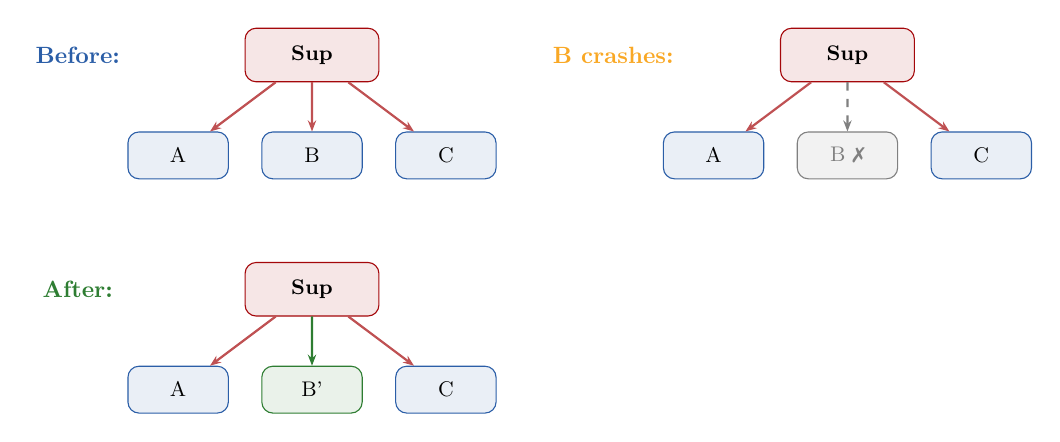
\begin{tikzpicture}[scale=0.85, every node/.style={scale=0.85},
    sup/.style={draw=erlred, fill=erlred!10, rounded corners=4pt,
                minimum width=2cm, minimum height=0.8cm, font=\small\bfseries},
    wrk/.style={draw=erlblue, fill=erlblue!10, rounded corners=4pt,
                minimum width=1.5cm, minimum height=0.7cm, font=\small},
    dead/.style={draw=gray, fill=gray!10, rounded corners=4pt,
                 minimum width=1.5cm, minimum height=0.7cm, font=\small, text=gray},
    new/.style={draw=erlgreen, fill=erlgreen!10, rounded corners=4pt,
                minimum width=1.5cm, minimum height=0.7cm, font=\small},
    link/.style={-{Stealth[length=4pt]}, thick, erlred!70},
]
    % Before
    \node[font=\bfseries\color{erlblue}] at (-1.5, 1) {Before:};
    \node[sup] (s1) at (2, 1) {Sup};
    \node[wrk] (a1) at (0, -0.5) {A};
    \node[wrk] (b1) at (2, -0.5) {B};
    \node[wrk] (c1) at (4, -0.5) {C};
    \draw[link] (s1) -- (a1);
    \draw[link] (s1) -- (b1);
    \draw[link] (s1) -- (c1);

    % B crashes
    \node[font=\bfseries\color{erlyellow}] at (6.5, 1) {B crashes:};
    \node[sup] (s2) at (10, 1) {Sup};
    \node[wrk] (a2) at (8, -0.5) {A};
    \node[dead] (b2) at (10, -0.5) {B \ding{55}};
    \node[wrk] (c2) at (12, -0.5) {C};
    \draw[link] (s2) -- (a2);
    \draw[link, gray, dashed] (s2) -- (b2);
    \draw[link] (s2) -- (c2);

    % After
    \node[font=\bfseries\color{erlgreen}] at (-1.5, -2.5) {After:};
    \node[sup] (s3) at (2, -2.5) {Sup};
    \node[wrk] (a3) at (0, -4) {A};
    \node[new] (b3) at (2, -4) {B'};
    \node[wrk] (c3) at (4, -4) {C};
    \draw[link] (s3) -- (a3);
    \draw[link, erlgreen] (s3) -- (b3);
    \draw[link] (s3) -- (c3);
\end{tikzpicture}
\caption{one\_for\_one：只重启崩溃的 B}
\end{figure}

\begin{lstlisting}[style=erlangstyle]
init(_) ->
    SupFlags = #{strategy => one_for_one,
                 intensity => 5, period => 3600},
    ChildSpecs = [child(worker_a), child(worker_b), child(worker_c)],
    {ok, {SupFlags, ChildSpecs}}.
\end{lstlisting}

\subsection{one\_for\_all}

\textbf{一个子进程崩溃，所有子进程都被终止并重启}。适用于子进程之间强耦合的场景。

\begin{figure}[H]
\centering
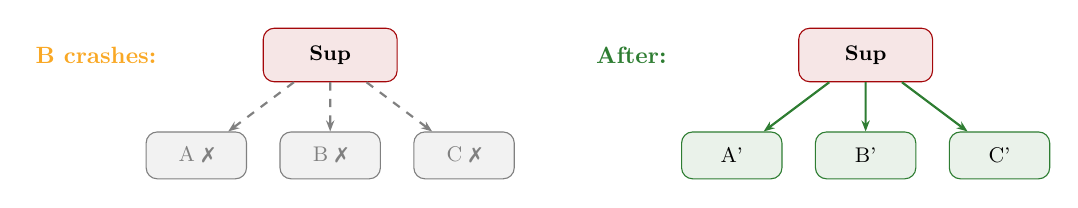
\begin{tikzpicture}[scale=0.85, every node/.style={scale=0.85},
    sup/.style={draw=erlred, fill=erlred!10, rounded corners=4pt,
                minimum width=2cm, minimum height=0.8cm, font=\small\bfseries},
    wrk/.style={draw=erlblue, fill=erlblue!10, rounded corners=4pt,
                minimum width=1.5cm, minimum height=0.7cm, font=\small},
    dead/.style={draw=gray, fill=gray!10, rounded corners=4pt,
                 minimum width=1.5cm, minimum height=0.7cm, font=\small, text=gray},
    new/.style={draw=erlgreen, fill=erlgreen!10, rounded corners=4pt,
                minimum width=1.5cm, minimum height=0.7cm, font=\small},
    link/.style={-{Stealth[length=4pt]}, thick, erlred!70},
]
    % B crashes
    \node[font=\bfseries\color{erlyellow}] at (-1.5, 1) {B crashes:};
    \node[sup] (s1) at (2, 1) {Sup};
    \node[dead] (a1) at (0, -0.5) {A \ding{55}};
    \node[dead] (b1) at (2, -0.5) {B \ding{55}};
    \node[dead] (c1) at (4, -0.5) {C \ding{55}};
    \draw[link, gray, dashed] (s1) -- (a1);
    \draw[link, gray, dashed] (s1) -- (b1);
    \draw[link, gray, dashed] (s1) -- (c1);

    % After: all restarted
    \node[font=\bfseries\color{erlgreen}] at (6.5, 1) {After:};
    \node[sup] (s2) at (10, 1) {Sup};
    \node[new] (a2) at (8, -0.5) {A'};
    \node[new] (b2) at (10, -0.5) {B'};
    \node[new] (c2) at (12, -0.5) {C'};
    \draw[link, erlgreen] (s2) -- (a2);
    \draw[link, erlgreen] (s2) -- (b2);
    \draw[link, erlgreen] (s2) -- (c2);
\end{tikzpicture}
\caption{one\_for\_all：B 崩溃后，A、B、C 全部重启}
\end{figure}

\subsection{rest\_for\_one}

\textbf{崩溃的子进程及其之后启动的所有子进程都被终止并重启}。适用于子进程之间有顺序依赖的场景。

\begin{figure}[H]
\centering
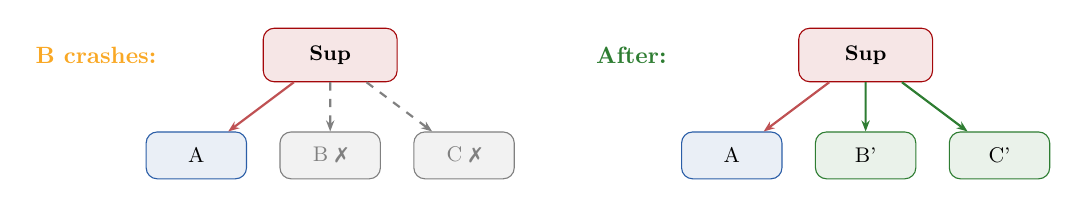
\begin{tikzpicture}[scale=0.85, every node/.style={scale=0.85},
    sup/.style={draw=erlred, fill=erlred!10, rounded corners=4pt,
                minimum width=2cm, minimum height=0.8cm, font=\small\bfseries},
    wrk/.style={draw=erlblue, fill=erlblue!10, rounded corners=4pt,
                minimum width=1.5cm, minimum height=0.7cm, font=\small},
    dead/.style={draw=gray, fill=gray!10, rounded corners=4pt,
                 minimum width=1.5cm, minimum height=0.7cm, font=\small, text=gray},
    new/.style={draw=erlgreen, fill=erlgreen!10, rounded corners=4pt,
                minimum width=1.5cm, minimum height=0.7cm, font=\small},
    link/.style={-{Stealth[length=4pt]}, thick, erlred!70},
]
    % B crashes
    \node[font=\bfseries\color{erlyellow}] at (-1.5, 1) {B crashes:};
    \node[sup] (s1) at (2, 1) {Sup};
    \node[wrk] (a1) at (0, -0.5) {A};
    \node[dead] (b1) at (2, -0.5) {B \ding{55}};
    \node[dead] (c1) at (4, -0.5) {C \ding{55}};
    \draw[link] (s1) -- (a1);
    \draw[link, gray, dashed] (s1) -- (b1);
    \draw[link, gray, dashed] (s1) -- (c1);

    % After: B and C restarted, A untouched
    \node[font=\bfseries\color{erlgreen}] at (6.5, 1) {After:};
    \node[sup] (s2) at (10, 1) {Sup};
    \node[wrk] (a2) at (8, -0.5) {A};
    \node[new] (b2) at (10, -0.5) {B'};
    \node[new] (c2) at (12, -0.5) {C'};
    \draw[link] (s2) -- (a2);
    \draw[link, erlgreen] (s2) -- (b2);
    \draw[link, erlgreen] (s2) -- (c2);
\end{tikzpicture}
\caption{rest\_for\_one：B 崩溃后，B 和 C 重启，A 不受影响}
\end{figure}

\begin{lstlisting}[style=erlangstyle, caption={rest\_for\_one 示例：frequency\_sup.erl}]
-module(frequency_sup).
-behaviour(supervisor).
-export([start_link/0, init/1]).

start_link() ->
    supervisor:start_link({local, ?MODULE}, ?MODULE, []).

init(_) ->
    ChildSpecList = [child(freq_overload), child(frequency)],
    {ok, {{rest_for_one, 2, 3600}, ChildSpecList}}.

child(Module) ->
    {Module, {Module, start_link, []},
     permanent, 2000, worker, [Module]}.
\end{lstlisting}

\begin{tipbox}[rest\_for\_one 的典型场景]
\texttt{frequency} 依赖 \texttt{freq\_overload}（事件管理器）。如果 \texttt{freq\_overload} 崩溃，\texttt{frequency} 也必须重启，因为它持有的事件管理器引用已失效。但如果 \texttt{frequency} 崩溃，\texttt{freq\_overload} 不需要重启。
\end{tipbox}

\subsection{simple\_one\_for\_one}

\textbf{所有子进程都是同一类型}，使用同一个 child spec 模板。子进程不在 \texttt{init/1} 中启动，而是通过 \texttt{supervisor:start\_child/2} 动态添加。

\begin{figure}[H]
\centering
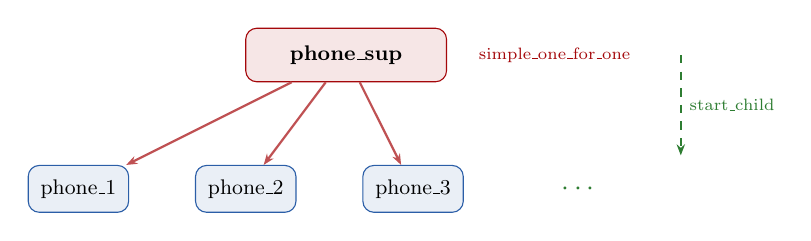
\begin{tikzpicture}[scale=0.85, every node/.style={scale=0.85},
    sup/.style={draw=erlred, fill=erlred!10, rounded corners=4pt,
                minimum width=3cm, minimum height=0.8cm, font=\small\bfseries},
    wrk/.style={draw=erlblue, fill=erlblue!10, rounded corners=4pt,
                minimum width=1.5cm, minimum height=0.7cm, font=\small},
    link/.style={-{Stealth[length=4pt]}, thick, erlred!70},
    add/.style={-{Stealth[length=4pt]}, thick, erlgreen, dashed},
]
    \node[sup] (s) at (4, 0) {phone\_sup};
    \node[font=\scriptsize\color{erlred}, right=3mm of s] {simple\_one\_for\_one};

    \node[wrk] (p1) at (0, -2) {phone\_1};
    \node[wrk] (p2) at (2.5, -2) {phone\_2};
    \node[wrk] (p3) at (5, -2) {phone\_3};
    \node[font=\large\color{erlgreen}] (dots) at (7.5, -2) {$\cdots$};

    \draw[link] (s) -- (p1);
    \draw[link] (s) -- (p2);
    \draw[link] (s) -- (p3);

    % Dynamic add arrow
    \draw[add] (9, 0) -- node[right, font=\scriptsize] {start\_child} (9, -1.5);
\end{tikzpicture}
\caption{simple\_one\_for\_one：动态添加同类子进程}
\end{figure}

\begin{lstlisting}[style=erlangstyle, caption={simple\_one\_for\_one 示例：simple\_phone\_sup.erl}]
-module(simple_phone_sup).
-behaviour(supervisor).
-export([start_link/0, attach_phone/1, detach_phone/1]).
-export([init/1]).

start_link() ->
    supervisor:start_link({local, ?MODULE}, ?MODULE, []).

init([]) ->
    {ok, {{simple_one_for_one, 10, 3600},
          [{ms, {phone_fsm, start_link, []},
            transient, 2000, worker, [phone_fsm]}]}}.

attach_phone(Ms) ->
    case hlr:lookup_id(Ms) of
        {ok, _Pid} -> {error, attached};
        _NotAttached ->
            supervisor:start_child(?MODULE, [Ms])
    end.

detach_phone(Ms) ->
    case hlr:lookup_id(Ms) of
        {ok, Pid} ->
            supervisor:terminate_child(?MODULE, Pid);
        _NotAttached ->
            {error, detached}
    end.
\end{lstlisting}

\begin{notebox}[simple\_one\_for\_one 的特殊之处]
\begin{itemize}[leftmargin=1.5em]
    \item \texttt{init/1} 中只能有\textbf{一个} child spec（作为模板）
    \item 初始化时\textbf{不启动}任何子进程
    \item 通过 \texttt{supervisor:start\_child(Sup, ExtraArgs)} 动态添加
    \item \texttt{ExtraArgs} 会追加到模板中的 \texttt{A} 参数后面：\texttt{apply(M, F, A ++ ExtraArgs)}
    \item 子进程的 id 都是 \texttt{undefined}，通过 PID 来区分
\end{itemize}
\end{notebox}

\subsection{策略对比}

\begin{table}[H]
\centering
\begin{tabular}{@{}llll@{}}
\toprule
\textbf{策略} & \textbf{崩溃影响范围} & \textbf{子进程关系} & \textbf{典型场景} \\
\midrule
\texttt{one\_for\_one} & 仅崩溃的进程 & 独立 & 通用场景 \\
\texttt{one\_for\_all} & 所有子进程 & 强耦合 & 共享状态 \\
\texttt{rest\_for\_one} & 崩溃的及之后的 & 顺序依赖 & 管道/依赖链 \\
\texttt{simple\_one\_for\_one} & 仅崩溃的进程 & 同类动态 & 连接池/会话 \\
\bottomrule
\end{tabular}
\caption{四种重启策略对比}
\end{table}


% ============================================================
% Section 5: Dynamic Child Management
% ============================================================
\section{动态子进程管理}

\subsection{supervisor API}

\begin{table}[H]
\centering
\begin{tabular}{@{}ll@{}}
\toprule
\textbf{函数} & \textbf{说明} \\
\midrule
\texttt{supervisor:start\_child(Sup, ChildSpec)} & 动态添加并启动子进程 \\
\texttt{supervisor:terminate\_child(Sup, Id)} & 终止子进程（保留 spec） \\
\texttt{supervisor:restart\_child(Sup, Id)} & 重启已终止的子进程 \\
\texttt{supervisor:delete\_child(Sup, Id)} & 删除已终止子进程的 spec \\
\texttt{supervisor:which\_children(Sup)} & 列出所有子进程 \\
\texttt{supervisor:count\_children(Sup)} & 统计子进程数量 \\
\bottomrule
\end{tabular}
\caption{supervisor 动态管理 API}
\end{table}

\subsection{动态添加子进程（one\_for\_one）}

\begin{lstlisting}[style=erlangstyle, caption={phone\_sup.erl --- 动态添加完整 ChildSpec}]
-module(phone_sup).
-behaviour(supervisor).
-export([start_link/0, attach_phone/1, detach_phone/1]).
-export([init/1]).

start_link() ->
    supervisor:start_link({local, ?MODULE}, ?MODULE, []).

init([]) ->
    {ok, {{one_for_one, 10, 3600}, []}}.  %% Empty child list

attach_phone(Ms) ->
    ChildSpec = {Ms, {phone_fsm, start_link, [Ms]},
                 transient, 2000, worker, [phone_fsm]},
    supervisor:start_child(?MODULE, ChildSpec).

detach_phone(Ms) ->
    supervisor:terminate_child(?MODULE, Ms),
    supervisor:delete_child(?MODULE, Ms).
\end{lstlisting}

\begin{tipbox}[one\_for\_one vs simple\_one\_for\_one 动态子进程]
\begin{itemize}[leftmargin=1.5em]
    \item \texttt{one\_for\_one}：\texttt{start\_child} 传入\textbf{完整的 ChildSpec}，每个子进程有唯一 Id
    \item \texttt{simple\_one\_for\_one}：\texttt{start\_child} 只传入\textbf{额外参数}，所有子进程共享同一模板
    \item \texttt{one\_for\_one} 可以 \texttt{restart\_child(Id)} 和 \texttt{delete\_child(Id)}
    \item \texttt{simple\_one\_for\_one} 只能 \texttt{terminate\_child(Pid)}，不支持 restart/delete
\end{itemize}
\end{tipbox}

\subsection{实验演示}

\begin{lstlisting}[style=shellstyle, caption={动态子进程管理实验}]
1> frequency_sup:start_link().
{ok,<0.60.0>}
2> whereis(frequency).
<0.62.0>
3> whereis(freq_overload).
<0.61.0>
4> frequency:stop().
ok
5> whereis(frequency).
<0.66.0>
6> exit(whereis(frequency), kill).
true
7> whereis(frequency).
<0.69.0>
8> supervisor:which_children(frequency_sup).
[{frequency,<0.69.0>,worker,[frequency]},
 {freq_overload,<0.61.0>,worker,[freq_overload]}]
9> supervisor:count_children(frequency_sup).
[{specs,2},{active,2},{supervisors,0},{workers,2}]
\end{lstlisting}

\begin{notebox}[观察]
\begin{itemize}[leftmargin=1.5em]
    \item 命令 4：\texttt{frequency:stop()} 正常停止 frequency，supervisor 自动重启（PID 从 62 变为 66）
    \item 命令 6：\texttt{exit(Pid, kill)} 强制杀死 frequency，supervisor 再次重启（PID 从 66 变为 69）
    \item 命令 8：\texttt{which\_children} 显示当前所有子进程及其 PID
    \item 命令 9：\texttt{count\_children} 显示统计信息
\end{itemize}
\end{notebox}


% ============================================================
% Section 6: Supervisor Bridge
% ============================================================
\section{Supervisor Bridge}

\subsection{什么是 supervisor\_bridge？}

\texttt{supervisor\_bridge} 用于将\textbf{非 OTP 兼容的进程}纳入监督树。当你有一个不遵循 OTP 行为模式的进程（如使用原始 \texttt{spawn} 创建的进程），可以通过 supervisor\_bridge 将其包装。

\begin{figure}[H]
\centering
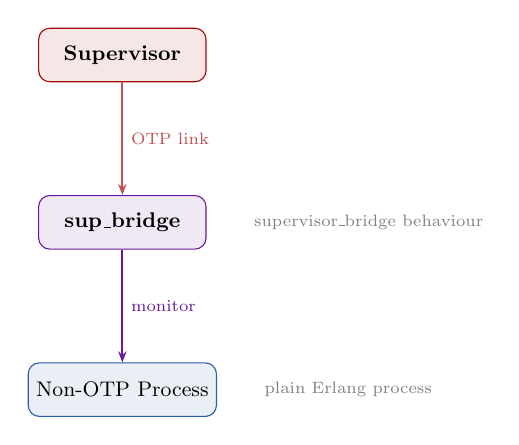
\begin{tikzpicture}[scale=0.85, every node/.style={scale=0.85},
    sup/.style={draw=erlred, fill=erlred!10, rounded corners=4pt,
                minimum width=2.5cm, minimum height=0.8cm, font=\small\bfseries},
    bridge/.style={draw=erlpurple, fill=erlpurple!10, rounded corners=4pt,
                   minimum width=2.5cm, minimum height=0.8cm, font=\small\bfseries},
    wrk/.style={draw=erlblue, fill=erlblue!10, rounded corners=4pt,
                minimum width=2.5cm, minimum height=0.8cm, font=\small},
    link/.style={-{Stealth[length=4pt]}, thick, erlred!70},
]
    \node[sup] (sup) at (3, 0) {Supervisor};
    \node[bridge] (bridge) at (3, -2.5) {sup\_bridge};
    \node[wrk] (proc) at (3, -5) {Non-OTP Process};

    \draw[link] (sup) -- node[right, font=\scriptsize] {OTP link} (bridge);
    \draw[link, erlpurple] (bridge) -- node[right, font=\scriptsize] {monitor} (proc);

    \node[font=\scriptsize\color{gray}, right=5mm of bridge] {supervisor\_bridge behaviour};
    \node[font=\scriptsize\color{gray}, right=5mm of proc] {plain Erlang process};
\end{tikzpicture}
\caption{supervisor\_bridge 架构}
\end{figure}

\subsection{回调函数}

\begin{lstlisting}[style=erlangstyle]
-behaviour(supervisor_bridge).
-export([init/1, terminate/2]).

%% init/1: Start the non-OTP process, return its Pid
init(Args) ->
    {ok, Pid, State}   %% Pid = the process to monitor
  | ignore
  | {error, Reason}.

%% terminate/2: Stop the non-OTP process
terminate(Reason, State) ->
    %% Clean up the non-OTP process
    ok.
\end{lstlisting}

\subsection{示例：包装 frequency 进程}

\begin{lstlisting}[style=erlangstyle, caption={frequency\_sup\_bridge.erl}]
-module(frequency_sup_bridge).
-behaviour(supervisor_bridge).
-export([start_link/0]).
-export([init/1, terminate/2]).

-define(PROCESS_NAME, frequency).

start_link() ->
    supervisor_bridge:start_link(
        {local, ?MODULE}, ?MODULE, []).

init([]) ->
    ?PROCESS_NAME:start_link(),
    case whereis(?PROCESS_NAME) of
        Pid when is_pid(Pid) -> {ok, Pid, []};
        undefined -> {error, start_error}
    end.

terminate(_Reason, []) ->
    ?PROCESS_NAME:stop().
\end{lstlisting}


% ============================================================
% Section 7: Nested Supervisors
% ============================================================
\section{嵌套监督树}

\subsection{多层监督树}

在实际应用中，通常需要多层 supervisor 来组织不同的子系统：

\begin{lstlisting}[style=erlangstyle, caption={bsc\_sup.erl --- 顶层 supervisor}]
-module(bsc_sup).
-behaviour(supervisor).
-export([start_link/0, init/1]).

start_link() ->
    supervisor:start_link({local, ?MODULE}, ?MODULE, []).

init(_) ->
    ChildSpecList = [
        child(freq_overload),
        child(frequency),
        child(simple_phone_sup)  %% Sub-supervisor!
    ],
    {ok, {{rest_for_one, 2, 3600}, ChildSpecList}}.

child(Module) ->
    {Module, {Module, start_link, []},
     permanent, 2000, worker, [Module]}.
\end{lstlisting}

\begin{warnbox}[注意：子 supervisor 的 type]
当子进程是另一个 supervisor 时，应该将 \texttt{type} 设为 \texttt{supervisor}，\texttt{shutdown} 设为 \texttt{infinity}：
\begin{lstlisting}[style=erlangstyle]
child_supervisor(Module) ->
    #{id => Module,
      start => {Module, start_link, []},
      restart => permanent,
      shutdown => infinity,    %% Wait for sub-tree to shut down
      type => supervisor,      %% Mark as supervisor
      modules => [Module]}.
\end{lstlisting}
\end{warnbox}

\subsection{监督树设计原则}

\begin{enumerate}[leftmargin=2em]
    \item \textbf{隔离故障域}：将相关的进程放在同一个 supervisor 下
    \item \textbf{选择合适的策略}：根据子进程之间的依赖关系选择重启策略
    \item \textbf{控制重启频率}：合理设置 intensity 和 period
    \item \textbf{启动顺序}：被依赖的进程排在前面
    \item \textbf{关闭超时}：给子进程足够的时间优雅关闭
    \item \textbf{层次化}：使用子 supervisor 构建多层树，避免单个 supervisor 管理过多子进程
\end{enumerate}


% ============================================================
% Section 8: auto_shutdown (OTP 24+)
% ============================================================
\section{auto\_shutdown（OTP 24+）}

\subsection{概念}

\texttt{auto\_shutdown} 允许 supervisor 在特定条件下自动关闭自身。这对于管理一组临时任务特别有用。

\begin{lstlisting}[style=erlangstyle]
SupFlags = #{
    strategy => one_for_all,
    intensity => 0,
    period => 1,
    auto_shutdown => any_significant  %% OTP 24+
}.
\end{lstlisting}

\subsection{auto\_shutdown 选项}

\begin{table}[H]
\centering
\begin{tabular}{@{}ll@{}}
\toprule
\textbf{值} & \textbf{说明} \\
\midrule
\texttt{never} & 默认值，supervisor 不会自动关闭 \\
\texttt{any\_significant} & 任何一个 \texttt{significant} 子进程正常终止时关闭 \\
\texttt{all\_significant} & 所有 \texttt{significant} 子进程都正常终止时关闭 \\
\bottomrule
\end{tabular}
\caption{auto\_shutdown 选项}
\end{table}

\subsection{significant 子进程}

在 child spec 中设置 \texttt{significant => true}：

\begin{lstlisting}[style=erlangstyle]
ChildSpec = #{
    id => main_task,
    start => {task_module, start_link, []},
    restart => temporary,
    significant => true    %% Mark as significant
}.
\end{lstlisting}

\begin{notebox}[使用限制]
\begin{itemize}[leftmargin=1.5em]
    \item \texttt{significant => true} 只能用于 \texttt{restart => temporary} 或 \texttt{restart => transient} 的子进程
    \item \texttt{auto\_shutdown} 不能与 \texttt{simple\_one\_for\_one} 策略一起使用
\end{itemize}
\end{notebox}


% ============================================================
% Section 9: Best Practices
% ============================================================
\section{最佳实践与常见陷阱}

\subsection{最佳实践}

\begin{enumerate}[leftmargin=2em]
    \item \textbf{使用 start\_link}：子进程必须使用 \texttt{start\_link} 而非 \texttt{start}，确保与 supervisor 链接
    \item \textbf{合理设置 shutdown}：worker 默认 5000ms，supervisor 用 \texttt{infinity}
    \item \textbf{trap\_exit}：如果子进程需要在终止时执行清理操作，设置 \texttt{process\_flag(trap\_exit, true)}
    \item \textbf{避免在 init/1 中做耗时操作}：supervisor 的 \texttt{start\_link} 是同步的，\texttt{init/1} 中的耗时操作会阻塞整个启动流程。使用 \texttt{\{continue, post\_init\}} 延迟初始化
    \item \textbf{使用 Map 格式}：OTP 18+ 推荐使用 Map 格式的 SupFlags 和 ChildSpec
    \item \textbf{合理设置重启频率}：太高会导致无限重启，太低会导致 supervisor 过早终止
    \item \textbf{使用 observer}：\texttt{observer:start()} 可以可视化监督树
\end{enumerate}

\subsection{常见陷阱}

\subsubsection{陷阱 1：使用 start 而非 start\_link}

\begin{lstlisting}[style=erlangstyle]
%% BAD: child not linked to supervisor
child(Module) ->
    {Module, {Module, start, []},  %% start, not start_link!
     permanent, 2000, worker, [Module]}.

%% GOOD: child linked to supervisor
child(Module) ->
    {Module, {Module, start_link, []},
     permanent, 2000, worker, [Module]}.
\end{lstlisting}

\subsubsection{陷阱 2：init/1 中的耗时操作}

\begin{lstlisting}[style=erlangstyle]
%% BAD: blocks supervisor startup
init(Args) ->
    Data = expensive_database_query(),  %% Blocks!
    {ok, Data}.

%% GOOD: use handle_continue for deferred init
init(Args) ->
    {ok, #{}, {continue, post_init}}.

handle_continue(post_init, State) ->
    Data = expensive_database_query(),
    {noreply, State#{data => Data}}.
\end{lstlisting}

\subsubsection{陷阱 3：重启频率设置不当}

\begin{lstlisting}[style=erlangstyle]
%% BAD: too permissive, may restart forever
#{intensity => 1000, period => 1}

%% BAD: too strict, supervisor dies on first restart
#{intensity => 0, period => 1}

%% GOOD: reasonable defaults
#{intensity => 5, period => 3600}
\end{lstlisting}

\subsubsection{陷阱 4：忘记处理 shutdown 信号}

\begin{lstlisting}[style=erlangstyle]
%% BAD: child ignores shutdown signal
init(Args) ->
    %% No trap_exit, terminate/2 won't be called
    {ok, State}.

%% GOOD: trap exit to handle graceful shutdown
init(Args) ->
    process_flag(trap_exit, true),
    {ok, State}.

terminate(Reason, State) ->
    %% Clean up resources
    close_connections(State),
    ok.
\end{lstlisting}

\subsubsection{陷阱 5：子 supervisor 的 shutdown 不是 infinity}

\begin{lstlisting}[style=erlangstyle]
%% BAD: sub-supervisor may be killed before children shut down
{sub_sup, {sub_sup, start_link, []},
 permanent, 2000, supervisor, [sub_sup]}.

%% GOOD: give sub-supervisor infinite time
{sub_sup, {sub_sup, start_link, []},
 permanent, infinity, supervisor, [sub_sup]}.
\end{lstlisting}


% ============================================================
% Section 10: Quick Reference
% ============================================================
\section{快速参考}

\subsection{启动函数}

\begin{table}[H]
\centering
\begin{tabular}{@{}ll@{}}
\toprule
\textbf{函数} & \textbf{说明} \\
\midrule
\texttt{supervisor:start\_link(Mod, Args)} & 启动不注册 \\
\texttt{supervisor:start\_link(\{local,N\}, Mod, Args)} & 启动并本地注册 \\
\texttt{supervisor:start\_link(\{global,N\}, Mod, Args)} & 启动并全局注册 \\
\bottomrule
\end{tabular}
\caption{启动函数}
\end{table}

\subsection{子进程管理函数}

\begin{table}[H]
\centering
\begin{tabular}{@{}ll@{}}
\toprule
\textbf{函数} & \textbf{说明} \\
\midrule
\texttt{supervisor:start\_child(Sup, ChildSpec)} & 动态添加并启动子进程 \\
\texttt{supervisor:terminate\_child(Sup, Id)} & 终止子进程 \\
\texttt{supervisor:restart\_child(Sup, Id)} & 重启已终止的子进程 \\
\texttt{supervisor:delete\_child(Sup, Id)} & 删除子进程规格 \\
\texttt{supervisor:which\_children(Sup)} & 列出所有子进程 \\
\texttt{supervisor:count\_children(Sup)} & 统计子进程数量 \\
\bottomrule
\end{tabular}
\caption{子进程管理函数}
\end{table}

\subsection{回调函数}

\begin{lstlisting}[style=erlangstyle]
%% supervisor callback
init(Args) ->
    {ok, {SupFlags, [ChildSpec, ...]}}
  | ignore.

%% SupFlags (map format, OTP 18+)
#{strategy => Strategy,
  intensity => MaxRestarts,
  period => Seconds,
  auto_shutdown => never | any_significant | all_significant}.

%% ChildSpec (map format, OTP 18+)
#{id => Id,
  start => {M, F, A},
  restart => permanent | transient | temporary,
  significant => boolean(),
  shutdown => brutal_kill | Timeout | infinity,
  type => worker | supervisor,
  modules => [Module] | dynamic}.
\end{lstlisting}

\subsection{重启策略速查}

\begin{table}[H]
\centering
\begin{tabular}{@{}lll@{}}
\toprule
\textbf{策略} & \textbf{B 崩溃时} & \textbf{适用场景} \\
\midrule
\texttt{one\_for\_one} & 只重启 B & 子进程独立 \\
\texttt{one\_for\_all} & 重启 A, B, C & 子进程强耦合 \\
\texttt{rest\_for\_one} & 重启 B, C（A 不动） & 顺序依赖 \\
\texttt{simple\_one\_for\_one} & 只重启 B & 同类动态子进程 \\
\bottomrule
\end{tabular}
\caption{重启策略速查（假设启动顺序为 A, B, C）}
\end{table}

\subsection{参考源码文件}

\begin{table}[H]
\centering
\begin{tabular}{@{}ll@{}}
\toprule
\textbf{文件} & \textbf{说明} \\
\midrule
\texttt{my\_supervisor.erl} & 手动实现的简单 supervisor \\
\texttt{frequency\_sup.erl} & rest\_for\_one 策略示例 \\
\texttt{frequency\_sup2.erl} & 带事件处理器的 supervisor \\
\texttt{bsc\_sup.erl} & 嵌套监督树示例 \\
\texttt{simple\_phone\_sup.erl} & simple\_one\_for\_one 策略示例 \\
\texttt{phone\_sup.erl} & one\_for\_one 动态子进程示例 \\
\texttt{frequency\_sup\_bridge.erl} & supervisor\_bridge 示例 \\
\texttt{frequency.erl} & gen\_server worker 示例 \\
\texttt{freq\_overload.erl} & gen\_event worker 示例 \\
\bottomrule
\end{tabular}
\caption{参考源码文件}
\end{table}

\subsection{Makefile 命令}

\begin{lstlisting}[style=shellstyle, caption={doc/Makefile 可用命令}]
make              # Compile and generate PDF
make pdf          # Same as above
make draft        # Quick single-pass PDF
make view         # Compile and open PDF
make stats        # Show document statistics
make clean        # Remove intermediate files
make distclean    # Remove all generated files
\end{lstlisting}


\end{document}
